\documentclass{book}

\usepackage[T1]{fontenc}
\usepackage[UTF8]{inputenc}
\usepackage{amsmath}
\usepackage{amsfonts}
\usepackage{amssymb}
\usepackage{stmaryrd}
\usepackage{lmodern}
\usepackage{ngerman}
\usepackage{xcolor}
\usepackage{geometry}
\usepackage[siunitx]{circuitikz}
\usepackage{tikz-cd}
\usepackage{makeidx}
\usepackage{hyperref}

\newcommand{\klam}[1]{\left(#1\right)}
\newcommand{\set}[2]{\left\lbrace #1~|~#2 \right\rbrace}
\newcommand{\grp}[2]{\left\langle #1~|~#2 \right\rangle}

\newcommand{\Def}[1]{\subsection{Definition: #1}}
\newcommand{\Bsp}[1]{\subsection{Beispiel: #1}}
\newcommand{\Lem}[1]{\subsection{Lemma: #1}}
\newcommand{\Bem}[1]{\subsection{Bemerkung: #1}}
\newcommand{\Kor}[1]{\subsection{Korollar: #1}}
\newcommand{\Satz}[1]{\subsection{Satz: #1}}

\newenvironment{Beweis}[1]{\paragraph{Beweis: \glqq #1\grqq\\}}{\hfill $\square$}

\renewcommand{\i}{^{-1}}

\renewcommand{\d}{\partial}

\newcommand{\C}{\mathcal{C}}
\newcommand{\D}{\mathcal{D}}
\newcommand{\F}{\mathcal{F}}
\newcommand{\G}{\mathcal{G}}
\newcommand{\I}{\mathcal{I}}
\renewcommand{\O}{\mathcal{O}}
\renewcommand{\H}{\widetilde{H}}
\newcommand{\R}{\mathbb{R}}
\newcommand{\N}{\mathbb{N}}

\newcommand{\e}{\varepsilon}
\newcommand{\inc}[2]{\textsf{inc}^{#1}_{#2}}

\newcommand{\Coprod}[1]{\underset{#1}{\coprod}}
\newcommand{\Oplus}[1]{\underset{#1}{\bigoplus}}

\newcommand{\colim}[1]{\underset{#1}{\textsf{colim}}}
\newcommand{\id}[1]{\textsf{id}_{#1}}
\newcommand{\df}[1]{\textbf{#1}\index{#1}}
\newcommand{\Z}{\mathbb{Z}}
\newcommand{\Top}{\textbf{Top}}
\newcommand{\Mod}{\textbf{Mod}}
\newcommand{\Set}{\textbf{Set}}
\newcommand{\Grp}{\textbf{Grp}}
\newcommand{\GRP}{\textbf{Gruppoid}}
\newcommand{\CovB}{\textbf{Cov}_B}
\newcommand{\Cov}[1]{\textbf{Cov}_{#1}}
\newcommand{\Hom}[3]{\textsf{Hom}_{#1}\left(#2, #3\right)}
\newcommand{\HomC}[2]{\Hom{\C}{#1}{#2}}
\newcommand{\Aut}[2]{\textsf{Aut}_{#1}\left(#2\right)}
\newcommand{\Ker}{\textsf{Kern}}
\newcommand{\Coker}{\textsf{Kokern}}
\newcommand{\Img}{\textsf{Bild}}

\newcommand{\Pfeil}[1]{\overset{#1}{\longrightarrow}}
\newcommand{\Lpfeil}[1]{\overset{#1}{\longleftarrow}}
\newcommand{\pfeil}[1]{\overset{#1}{\rightarrow}}
\newcommand{\lpfeil}[1]{\overset{#1}{\leftarrow}}
\newcommand{\inj}[1]{\overset{#1}{\hookrightarrow}}
\newcommand{\linj}[1]{\overset{#1}{\hookleftarrow}}
\newcommand{\Inj}[1]{\overset{#1}{\hookrightarrow}}
\newcommand{\Linj}[1]{\overset{#1}{\hookleftarrow}}
\newcommand{\impl}[1]{\overset{#1}{\Rightarrow}}
\newcommand{\Impl}[1]{\overset{#1}{\Longrightarrow}}

\newcommand{\off}{\overset{o}{\subset}}
\newcommand{\abg}{\overset{c}{\subset}}

\newcommand{\Hs}[1]{H^{sing}_{#1}}
\newcommand{\Cs}[1]{C^{sing}_{#1}}
\newcommand{\cs}[1]{c^{sing}_{#1}}
\newcommand{\Hw}[1]{H^{CW}_{#1}}
\newcommand{\Cw}[1]{C^{CW}_{#1}}
\newcommand{\cw}[1]{c^{CW}_{#1}}

\newcommand{\func}[5]{
\begin{align*}
#1 : #2 & \longrightarrow #3\\
#4 & \longmapsto #5
\end{align*}
}

\newcommand{\diag}[8]{
\begin{tikzpicture}
\node (D1) at (0,2) [] {$#1$};
\node (D3) at (2,2) [] {$#3$};
\node (D5) at (2,0) [] {$#5$};
\node (D7) at (0,0) [] {$#7$};

\draw [->] (D1) -> (D3) node[midway, above] {$#2$};
\draw [->] (D3) -> (D5) node[midway, right] {$#4$};
\draw [->] (D7) -> (D5) node[midway, below] {$#6$};
\draw [->] (D1) -> (D7) node[midway, left] {$#8$};

\end{tikzpicture}
}
\newcommand{\Diag}[8]{
\begin{tikzpicture}
\node (D1) at (0,2) [] {$#1$};
\node (D3) at (4,2) [] {$#3$};
\node (D5) at (4,0) [] {$#5$};
\node (D7) at (0,0) [] {$#7$};

\draw [->] (D1) -> (D3) node[midway, above] {$#2$};
\draw [->] (D3) -> (D5) node[midway, right] {$#4$};
\draw [->] (D7) -> (D5) node[midway, below] {$#6$};
\draw [->] (D1) -> (D7) node[midway, left] {$#8$};

\end{tikzpicture}
}

\newcommand{\triag}[6]{
\begin{tikzpicture}
\node (D1) at (0,2) [] {$#1$};
\node (D3) at (2,2) [] {$#3$};
\node (D5) at (1,0) [] {$#5$};

\draw [->] (D1) -> (D3) node[midway, above] {$#2$};
\draw [->] (D3) -> (D5) node[midway, below right] {$#4$};
\draw [->] (D1) -> (D5) node[midway, below left] {$#6$};

\end{tikzpicture}
}

\begin{document}

% 1.VL 13.4.15
\chapter{Categorial Language and the van-Kampen theorem}
\section{Kategorien}
\section{Funktoren}
\section{Natürliche Transformationen}
\Def{Natürliche Transformationen}
Sind $\F, \G : \C \rightarrow \D$ Funktoren, so ist eine \df{natürliche Transformation} $\alpha : \F \rightarrow \G$ definiert durch Pfeile $\alpha_A : \F(A) \rightarrow \G(A)$ für alle $A \in \C$, sodass
\begin{center}
\diag{\F(A)}{\F(f)}{\F(B)}{\alpha_B}{\G(B)}{\G(f)}{\G(A)}{\alpha_A}
\end{center}
für alle $A, B \in \C, f \in \HomC{A}{B}$kommutiert.

\Def{Natürliche Isomorphien}
Eine \df{natürliche Isomorphie} ist eine natürliche Transformation $\alpha : \F \rightarrow \G$, bei der alle Pfeile $\alpha_A : \F(A) \rightarrow \G(A)$ isomorph sind.

%2.VL, 15.4.15

\Def{Äquivalenzen von Kategorien}
Kategorien $\C,\D$ heißen \df{natürlich äquivalent}, falls Funktoren $\F : \C \rightarrow \D, \G : \D\rightarrow \C$ existieren, sodass $\G\circ \F$ natürlich isomorph zu $\id{\C}$ und $\F\circ \G$ natürlich isomorph zu $\id{\D}$ sind.

\section{Adjungierte Funktoren}
\Def{Adjungierte}
Seien $\F : \C \rightarrow \D, \G : \D \rightarrow \C$ Funktoren. $\F$ heißt \df{linksadjungiert} zu $\G$ und $\G$ \df{rechtsadjungiert} zu $\F$, falls für alle $A \in \C, B \in \D$ gilt:
\[\HomC{A}{\G(B)} \cong \Hom{D}{\F(A)}{B} \]

\Def{Präsentation von Gruppen}
Sei $S$ eine Menge und $R$ eine Teilmenge von $S^*$. Wir definieren $\grp{S}{R}$ als die \df{Präsentation} $\G$, falls
\[\grp{S}{R} := \F(S)/ N(R) \cong G \]
$G$ ist \df{endlich präsentiert}, falls $S$ und $R$ endlich sind.

\section{Limes Konstruktionen}
\Def{Produkt}
Sind $X,Y \in \C$ Objekte einer Kategorie, so definieren wir das \df{Produkt} von $X$ und $Y$ als das größte Objekt $X\times Y$ zusammen mit Abbildungen $\pi_X : X\times Y \rightarrow X, \pi_Y : X\times Y \rightarrow Y$, sodass folgende UAE erfüllt wird:
\begin{center}
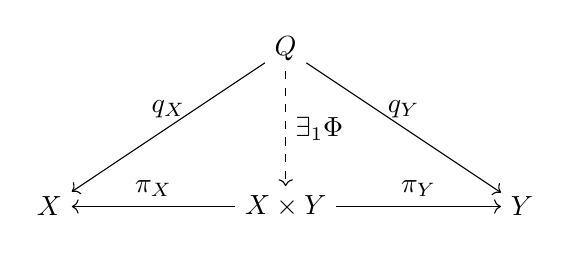
\begin{tikzpicture}
\node (Q) at (3,2) [] {$Q$};
\node (X) at (0,0) [] {$X$};
\node (XY) at (3,0) [] {$X\times Y$};
\node (Y) at (6,0) [] {$Y$};

\draw [->] (Q) -> (X) node[midway, above] {$q_X$};
\draw [->] (Q) -> (Y) node[midway, above] {$q_Y$};
\draw [->, dashed] (Q) -> (XY) node[midway, right] {$\exists_1 \Phi$};
\draw [->] (XY) -> (X) node[midway, above] {$\pi_X$};
\draw [->] (XY) -> (Y) node[midway, above] {$\pi_Y$};
\end{tikzpicture}
\end{center}

\Def{Pullback}
Seien $X,Y,Z\in\C$ Objekte einer Kategorie mit den Abbildungen $X \rightarrow Y \leftarrow Z$. Dann ist ein \df{Pullback} bzw. \df{Faserprodukt} $P$ das größte Objekt, das folgendes \df{Pullback-Diagramm} zum kommutieren bringt.
\begin{center}
\diag{P}{}{X}{}{Y}{}{Z}{}
\end{center}
d.h. es erfüllt folgende UAE:
\begin{center}
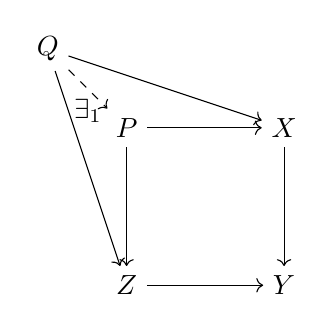
\begin{tikzpicture}
\node (Q) at (-1,3) [] {$Q$};
\node (D1) at (0,2) [] {$P$};
\node (D3) at (2,2) [] {$X$};
\node (D5) at (2,0) [] {$Y$};
\node (D7) at (0,0) [] {$Z$};

\draw [->] (D1) -> (D3) node[midway, above] {};
\draw [->] (D3) -> (D5) node[midway, right] {};
\draw [->] (D7) -> (D5) node[midway, below] {};
\draw [->] (D1) -> (D7) node[midway, left] {};
\draw [->] (Q) -> (D3) node[midway, above] {};
\draw [->] (Q) -> (D7) node[midway, right] {};
\draw [->, dashed] (Q) -> (D1) node[midway, below] {$\exists_1$};

\end{tikzpicture}
\end{center}

\Bsp{Pullback}
In $\Set$ ist der Pullback gerade $X\times_S Y = \set{(x,y) \in X \times Y}{f(x) = g(y)}$ für $X \pfeil{f} S \lpfeil{g} Y$. In \Top ist der Pullback dieselbe Menge mit der entsprechenden Spurtopologie.

\Bsp{Überlagerung}
Sei $\CovB$ die Kategorie der Überlagerung von $B \in \Top$. Sei ferner $\phi : B' \pfeil{} B$ eine stetige Abbildung. Dann definieren wir einen Funktor $\Phi : \CovB \rightarrow \Cov{B'}$ auf Objekten $X \in \CovB$ durch den Pullback:
\begin{center}
\diag{\Phi(X)}{}{X}{}{B}{\phi}{B'}{}
\end{center}
Und auf Pfeilen $X \pfeil{f} Y$ durch die UAE des folgenden Pullbacks:

\begin{center}
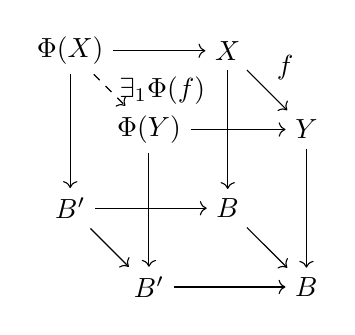
\begin{tikzpicture}
\node (C1) at (-1,3) [] {$\Phi(X)$};
\node (C3) at (1,3) [] {$X$};
\node (C5) at (1,1) [] {$B$};
\node (C7) at (-1,1) [] {$B'$};
\node (D1) at (0,2) [] {$\Phi(Y)$};
\node (D3) at (2,2) [] {$Y$};
\node (D5) at (2,0) [] {$B$};
\node (D7) at (0,0) [] {$B'$};

\draw [->] (D1) -> (D3) node[midway, above] {};
\draw [->] (D3) -> (D5) node[midway, right] {};
\draw [->] (D7) -> (D5) node[midway, below] {};
\draw [->] (D1) -> (D7) node[midway, left] {};
\draw [->] (C1) -> (C3) node[midway, above] {};
\draw [->] (C3) -> (C5) node[midway, right] {};
\draw [->] (C7) -> (C5) node[midway, below] {};
\draw [->] (C1) -> (C7) node[midway, left] {};
\draw [->, dashed] (C1) -> (D1) node[midway, right] {$\exists_1\Phi(f)$};
\draw [->] (C3) -> (D3) node[midway, above right] {$f$};
\draw [->] (C5) -> (D5) node[midway, below] {};
\draw [->] (C7) -> (D7) node[midway, left] {};
\end{tikzpicture}
\end{center}

% 22.4, 4. VL

\Def{Diagramme}
Ein \df{Diagramm} der Gestalt $\I$ ist ein Funktor von einer kleinen Kategorie $\I$ in eine Kategorie.

\Def{Kegel}
Der \df{Kegel} eines Diagrammes $\D : \I \rightarrow \C$ ist ein Objekt $A \in \C$ mit einer Familie von Pfeilen $\klam{A \rightarrow \D(i)}_{i\in \I}$, sodass folgendes Dreieck
\begin{center}
\triag{A}{}{\D(i)}{\D(g)}{\D(j)}{}
\end{center}
für alle Pfeile $i\pfeil{g} j$ in $\I$ kommutiert.

\Def{Limes}
Der \df{Limes} eines Diagrammes $\D : \I \rightarrow \C$ ist der größte Kegel $L \in \C$, d.h. es erfüllt folgende UAE für alle Kegel $A$ von $D$
\begin{center}
\triag{A}{\exists_1}{L}{}{\D(i)}{}
\end{center}
für alle $i\in\I$.

\Bsp{Limites}
\begin{itemize}
\item Das Produkt einer Kategorie ist der Limes eines Diagramms der Gestalt
\[ \bullet_1 ~~~~~~~~~~~ \bullet_2 \]
\item Der Pullback einer Kategorie ist der Limes eines Diagramms der Gestalt
\[ \bullet_1 \pfeil{} \bullet_2 \lpfeil{} \bullet_3 \]
\end{itemize}

\Def{Koprodukt}
Sind $X,Y \in \C$ Objekte einer Kategorie, so definieren wir das \df{Koprodukt} von $X$ und $Y$ als das kleinste Objekt $X\oplus Y$ zusammen mit Abbildungen $\iota_X : X\times Y \rightarrow X, \iota_Y : X\times Y \rightarrow Y$, sodass folgende UAE erfüllt wird:
\begin{center}
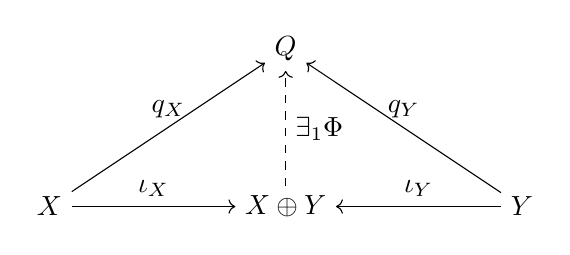
\begin{tikzpicture}
\node (Q) at (3,2) [] {$Q$};
\node (X) at (0,0) [] {$X$};
\node (XY) at (3,0) [] {$X\oplus Y$};
\node (Y) at (6,0) [] {$Y$};

\draw [->] (X) -> (Q) node[midway, above] {$q_X$};
\draw [->] (Y) -> (Q) node[midway, above] {$q_Y$};
\draw [->, dashed] (XY) -> (Q) node[midway, right] {$\exists_1 \Phi$};
\draw [->] (X) -> (XY) node[midway, above] {$\iota_X$};
\draw [->] (Y) -> (XY) node[midway, above] {$\iota_Y$};
\end{tikzpicture}
\end{center}

\Def{Freies Gruppenprodukt}
Das freie Produkt $G\star H$ ist definiert als das Koprodukt zweier Gruppen $G$ und $H$.

\Lem{Freies Gruppenprodukt}
In \Grp existieren Koprodukte und es gilt
\[ \grp{S_1}{R_1} \star \grp{S_2}{R_2} \cong \grp{S_1\sqcup S_2}{R_1 \sqcup R_2}\]

\Def{Pushout}
Seien $X,Y,Z\in\C$ Objekte einer Kategorie mit den Abbildungen $Y \lpfeil{} X \pfeil{} Z$. Dann ist ein \df{Pushout} bzw. \df{Kofaserprodukt} $P$ das kleinste Objekt, das folgendes \df{Pushout-Diagramm} zum kommutieren bringt.
\begin{center}
\diag{X}{}{Y}{}{P}{}{Z}{}
\end{center}
d.h. es erfüllt folgende UAE:
\begin{center}
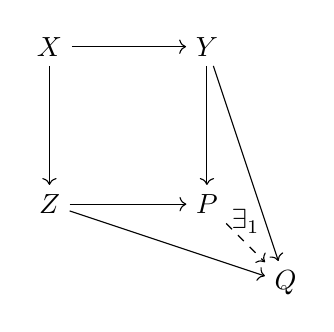
\begin{tikzpicture}
\node (Q) at (3,-1) [] {$Q$};
\node (D1) at (0,2) [] {$X$};
\node (D3) at (2,2) [] {$Y$};
\node (D5) at (2,0) [] {$P$};
\node (D7) at (0,0) [] {$Z$};

\draw [->] (D1) -> (D3) node[midway, above] {};
\draw [->] (D3) -> (D5) node[midway, right] {};
\draw [->] (D7) -> (D5) node[midway, below] {};
\draw [->] (D1) -> (D7) node[midway, left] {};
\draw [->] (D3) -> (Q) node[midway, above] {};
\draw [->] (D7) -> (Q) node[midway, right] {};
\draw [->, dashed] (D5) -> (Q) node[midway, above] {$\exists_1$};

\end{tikzpicture}
\end{center}

\Lem{Pushouts in \Top}
In $\Top$ existieren Pushouts und sind von der Gestalt
\begin{center}
\diag{A}{s}{X}{}{X\sqcup Y/\sim}{}{Y}{t}
\end{center}
wobei $\sim \subset X \times Y$ erzeugt wird durch
\[t(a) \sim s(a) ~~~\forall a \in A \]

\Def{Amalgiertes freies Produkt in \Grp}
Ist $G \hookleftarrow A \hookrightarrow H$ ein Diagramm von injektiven Gruppenhomomorphismen, so wird sein Pushout als \df{amalgiertes freies Produkt} $G\star_A H$ von $G, H$ über $A$ bezeichnet.

\Lem{Pushouts in \Grp}
Ist $G \linj{s} A \inj{t} H$, so existiert sein Pushout und ist von der Gestalt:
\[G\star_A H = G\star H/\set{s(a)t(a)^{-1}}{a \in A}\]

\Def{Kolimes}
Ist $\D : \I \pfeil{} \C$ ein Diagramm, so ist ein \df{Kolimes} ein Limes von $\D^\textsf{op}.$


\section{Der Fundamentalgruppoid}
\Def{Fundamentalgruppoid}
Ist $X$ ein topologischer Raum, dann definieren wir den \df{Fundamentalgruppoiden} $\Pi(X)$ wie folgt:
\begin{itemize}
\item Objekte sind alle Punkte $x \in X$
\item Pfeile von $x$ nach $y$ sind die Homotopieklassen von Wegen von $x$ nach $y$. Also
\[\Hom{\Pi(X)}{x}{y} = \set{\gamma : x \rightarrow y}{}/\sim\]
\item Die Komposition ist die Konkatenation von Wegen.
\end{itemize}

% %27.4.15, 5.VL

\Def{Gruppoid}
Eine Kategorie heißt \df{Gruppoid}, falls alle Pfeile isomorph sind.

\Def{Zusammenhängende Kategorien}
Eine Kategorie heißt \df{zusammenhängend}, falls jedes Paar von Objekten durch eine (nicht zwangsläufig gerichtete) Sequenz von Pfeilen verbunden werden kann.

\Lem{Einbettungsfunktor}
Ist $G$ ein zusammenhängender Gruppoid, dann ist der Einbettungsfunktor
\[\I_x : \Aut{G}{x} = \Hom{G}{x}{x} \longrightarrow \G \]
eine Äquivalenz von Kategorien für alle $x \in X$.

\Kor{}
Ist $X$ ein wegzusammenhängender Raum, so ist die Inklusion
\[\pi_{\klam{X,x}} \inj{} \Pi(X) \]
eine Äquivalenz von Kategorien für alle $x \in X$.

\section{Der Satz von Seifert-van Kampen}

\Bem{}
Wir definieren als \GRP\ die Kategorie der kleinen Gruppoide. Es existiert ein Einbettungsfunktor
\[\Grp \inj{} \GRP\]

\Satz{Der Satz von Seifert-van Kampen (kategorientheoretische Version)}
Sei $X$ ein topologischer Raum, $\O$ eine Überdeckung von $X$ durch offene Mengen, die abgeschlossen ist unter endlichen Schnitten.\\
Wir fassen $\O$ als eine Kategorie auf, deren Objekte die offenen Mengen und deren Pfeile Teilmengen-Inklusionen sind.\\
In diesem Fall erhalten wir einen Funktor
\begin{align*}
\Pi : \O & \longrightarrow  \GRP\\
U & \longmapsto  \Pi(U)\\
\klam{U\inj{\iota} V} & \longmapsto  \klam{\Pi(U) \pfeil{\Pi(\iota)} \Pi(V)}
\end{align*}
Dann gilt:
\[\Pi(X) = \colim{U \in \O}\Pi(U)\]

\Satz{Der Satz von Seifert-van Kampen}
Sei $X$ ein topologischer Raum, $x \in X$, $\O$ eine Überdeckung von $X$ durch offene, wegzusammenhängenden Mengen, die $x$ enthalten, die abgeschlossen ist unter endlichen Schnitten.\\
Dann ist $\pi_1(X,x)$ der Kolimes von
\begin{align*}
\pi_1(\_, x) : \O & \longrightarrow \Grp\\
U & \longmapsto  \pi_1(U, x)\\
\klam{U\inj{\iota} V} & \longmapsto  \klam{\pi_1(U,x) \pfeil{\pi_1(\iota,x)} \pi_1(V,x)}
\end{align*}
\[\pi_1(X,x) = \colim{U \in \O}\pi_1(U,x)\]

\begin{Beweis}{kategorischer SvK $\Rightarrow$ normaler SvK}
Wir beweisen die Aussage nur im Fall, dass $\O$ endlich ist.\\
Wir müssen zeigen, dass $\pi_1(X,x)$ die UAE des Kolimes von $\pi_1(\_, x)$ erfüllt.\\
Für jedes $U \in \O$ ist die Einbettung
\[\I_U : \pi_1(U,x) \longrightarrow \Pi(U) \]
eine Äquivalenz von Kategorien. Ein \textsl{inverser} Funktor $\F_U : \Pi(U) \rightarrow \pi_1(U,x)$ wird definiert durch eine Zuordnung
\[y \longmapsto [c_U^y]\]
Wir definieren $c_U^y$ induktiv für alle $U \in \O, y \in X$.
\begin{itemize}
\item Definiere $U_0 = \bigcap_{U\in \O}$. Ist $y \in U_0$, so bezeichne $c_{U_0}^y$ einen beliebigen Weg $x \mapsto y$ in $U_0$. $c_{U_0}^x$ bezeichne den konstanten Weg.
\item Existiert ein $V \in \O$, sodass $c_V^y$ bereits definiert und $V \subseteq U$ ist, so definiere $c_U^y := c_V^y$.\\
Anderenfalls definiere $c_U^y$ als beliebigen Pfad in $U$ von $x$ nach $y$.
\end{itemize}
Durch diese Wahl werden die Funktoren $\F_U$ verträglich im Sinne, dass folgende Diagramme für $U \subset V$ kommutieren
\begin{center}
\diag{\Pi(U)}{\F_U}{\pi_1(U,x)}{}{\pi_1(V,x)}{\F_V}{\Pi(V)}{}
\end{center}
Ergo kommutieren auch
\begin{center}
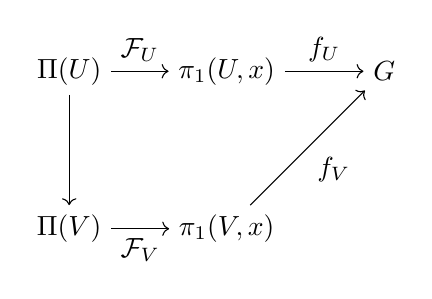
\begin{tikzpicture}
\node (D1) at (0,2) [] {$\Pi(U)$};
\node (D3) at (2,2) [] {$\pi_1(U,x)$};
\node (D5) at (2,0) [] {$\pi_1(V,x)$};
\node (D7) at (0,0) [] {$\Pi(V)$};
\node (D9) at (4,2) [] {$G$};

\draw [->] (D1) -> (D3) node[midway, above] {$\F_U$};
\draw [->] (D7) -> (D5) node[midway, below] {$\F_V$};
\draw [->] (D1) -> (D7) node[midway, left] {};
\draw [->] (D3) -> (D9) node[midway, above] {$f_U$};
\draw [->] (D5) -> (D9) node[midway, below right] {$f_V$};

\end{tikzpicture}
\end{center}
Die UAE von $\Pi(X)$ garantiert nun die Existenz eines eindeutig bestimmten Pfeils $f$, sodass folgende Diagramme kommutieren
\begin{center}
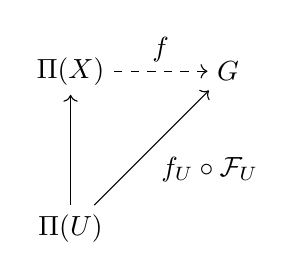
\begin{tikzpicture}
\node (U) at (0,0) [] {$\Pi(U)$};
\node (X) at (0,2) [] {$\Pi(X)$};
\node (G) at (2,2) [] {$G$};

\draw [->] (U) -> (X) node[midway, above] {};
\draw [->] (U) -> (G) node[midway, below right] {$f_U\circ \F_U$};
\draw [->, dashed] (X) -> (G) node[midway, above] {$f$};
\end{tikzpicture}
\end{center}
Ergo kommutieren auch folgende Diagramme
\begin{center}
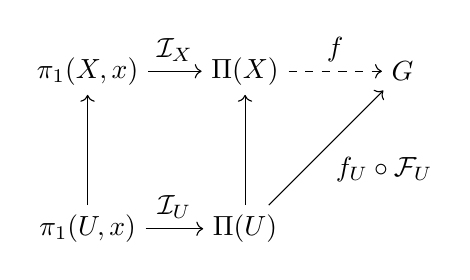
\begin{tikzpicture}
\node (u) at (-2,0) [] {$\pi_1(U,x)$};
\node (x) at (-2,2) [] {$\pi_1(X,x)$};
\node (U) at (0,0) [] {$\Pi(U)$};
\node (X) at (0,2) [] {$\Pi(X)$};
\node (G) at (2,2) [] {$G$};

\draw [->] (x) -> (X) node[midway, above] {$\I_X$};
\draw [->] (u) -> (U) node[midway, above] {$\I_U$};
\draw [->] (u) -> (x) node[midway, above] {};
\draw [->] (U) -> (X) node[midway, above] {};
\draw [->] (U) -> (G) node[midway, below right] {$f_U\circ \F_U$};
\draw [->, dashed] (X) -> (G) node[midway, above] {$f$};
\end{tikzpicture}
\end{center}
Da $\F_U \circ \I_U = \id{\pi_1(U,x)}$, erfüllt $\pi_1(X,x)$ die als Kolimes geforderte UAE.
\end{Beweis}

\Lem{Lebesgue Lemma}
Sei $X$ ein kompakter, metrischer Raum mit einer offenen Überdeckung durch $(U_i)_{i\in I}$. Dann existiert eine \df{Lebesgue Konstante} $\delta > 0$, sodass jede Teilmenge $A \subset X$ mit Durchmesser $< \delta$ komplett in einem $U_i$ enthalten ist.

% % % 29.4.15, 6. VL

\begin{Beweis}{kategorischer SvK}
Wir müssen zeigen, dass $\Pi(X)$ die UAE erfüllt, d.h. für jeden Kokegel $G$ existiert genau ein $\Pi(X) \pfeil{f} G$, sodass folgende Diagramme kommutieren:
\begin{center}
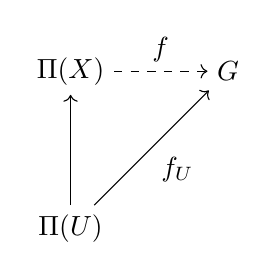
\begin{tikzpicture}
\node (U) at (0,0) [] {$\Pi(U)$};
\node (X) at (0,2) [] {$\Pi(X)$};
\node (G) at (2,2) [] {$G$};

\draw [->] (U) -> (X) node[midway, above] {};
\draw [->] (U) -> (G) node[midway, below right] {$f_U$};
\draw [->, dashed] (X) -> (G) node[midway, above] {$f$};
\end{tikzpicture}
\end{center}

Für $x \in U$, definieren wir
\[f(x) := f_U(x)\]
Ist $c$ ein Weg in $X$, so definieren wir
\[f([c]) :=f_U([c])\]
falls $c$ in einem $U$ enthalten ist. Ist $c$ beliebig, so ist $c^{-1}(\O)$ eine offene Überdeckung von $[0,1]$. Ergo existiert eine Lebesgue Konstante $\delta > 0$; wir unterteilen $[0,1]$ in $n$ viele Intervalle mit Länge $< \delta$ und erhalten eine Unterteilung von $c = c_1\cdots c_n$, wobei jedes $c_i$ in einem $U_j$ liegt. Folglich definieren wir nun
\[f([c]) = f([c_1]) \circ \ldots \circ f([c_n])\]
Es bleibt zu zeigen, dass die Definition von $f([c])$ unabhängig von der Wahl
\begin{enumerate}
\item[(i)] der Unterteilung von $[0,1]$ und
\item[(ii)] des Repräsentanten $c$ von $[c]$ ist.
\end{enumerate}
\end{Beweis}

\section{Anwendungen des Satzes von Seifert-van Kampen}
% % 7.VL 4.5.15
\Bem{Meistgenutzte Anwendung}
Ist $X = U\cup V$ mit $U, V \off X$, so erhalten wir folgendes Pushout Diagramm:
\begin{center}
\diag{U\cap V}{}{U}{}{X}{}{V}{}
\end{center}
Mit Seifert-van Kampen folgt nun für alle $x \in U\cap V$, dass $\pi_1(\_,x)$ Pushouts erhält:
\begin{center}
\diag{\pi_1(U\cap V,x)}{}{\pi_1(U,x)}{}{\pi_1(X,x)}{}{\pi_1(Y,x)}{}
\end{center}
Ergo
\[\pi_1(X,x) = \pi_1(U,x) \underset{\pi_1(V\cap U, x)}{\star} \pi_1(V,x)\]

\Satz{Anhängen von Zellen}
Sei $(S^{n-1}, *) \pfeil{f} (X,x)$ ein Pfeil, dann existiert folgender Pushout
\begin{center}
\diag{S^{n-1}}{f}{X}{j}{Y}{}{D^n}{\iota}
\end{center}
\begin{itemize}
\item Ist $n \geq 3$, dann ist $\pi_1(X,x) \pfeil{j_*} \pi_1(Y,j(x))$ ein Isomorphismus.
\item Ist $n = 2$, dann ist $j_*$ surjektiv und $\Ker j_*$ ist die normale Untegruppe, die von $[f]$ in $\pi_1(X,x)$ erzeugt wird.
\end{itemize}

\begin{Beweis}{}
Definiere $y = j(x), U = \overset{o}{D^n}, V = X \underset{f}{\cup}(D^n - 0)$. Dann ist $U\cap V \simeq S^{n-1}$
\begin{itemize}
\item Sei $y' \in U-0$ und $u$ ein Pfad in $Y$ von $y$ zu $y'$.\\
Für $n \geq 3$ ist $\pi_1(U\cap V, y') = 1$. Mit Seifert-van Kampen folgt:
\[\pi_1(Y,y') = \pi_1(U,y') \underset{\pi_1(U\cap V, y')}{\star} \pi_1(V, y') = \pi_1(V, y')\]
Da $y$ und $y'$ durch einen Weg verbunden werden, gilt:
\[\pi_1(V, y) \cong \pi_1(V, y')\]
Da $(V,y) \rightarrow (X,x)$ ein NDR ist, gilt schließlich
\[\pi_1(V, y) \cong \pi_1(X, x)\]

\item Ist $n = 2$, so ist $U\cap V \simeq S^1$. Mit Seifert-van Kampen folgt abermals
\[\pi_1(Y,y') = \pi_1(U,y') \underset{\pi_1(U\cap V, y')}{\star} \pi_1(V, y') = \pi_1(V, y') / N([f])\]
Da $f_*(\Z) = N([f])$.
\end{itemize}

\end{Beweis}

% % 6.5, 8.VL
\Bsp{Flächenwort}
Die orientierbare, geschlossene, zusammenhängende Fläche von Geschlecht $g$ ist definiert durch den Pushout
\begin{center}
\diag{S^1}{f}{\bigvee_{i=1}^{2g}S^1}{}{F_g}{}{D^2}{}
\end{center}
wobei wir die $2g$ Kreise in $\bigvee_{i=1}^{2g}S^1$ mit $a_1,b_1,\ldots,a_g, b_g$ bezeichnet werden. $f$ wird bestimmt durch das \df{Flächenwort} $\prod_{i=1}^{g}[a_i,b_i]$. Es folgt mit obigen Satz
\[\pi_1(F_g) = \grp{a_1,b_1,\ldots, a_g, b_g}{\prod_{i=1}^{g}[a_i,b_i]}\]


\Satz{}
Sei $G = \grp{S}{R}$ eine endlich präsentierte Gruppe. Dann existiert ein 2-dimensionaler Zellen-Komplex $(X,x)$ mit
\[\pi_1(X,x) \cong G\]

\section{Eigenschaften von Pushouts in \Top}
\Def{Identifizierungsabbildung}
$f : X \pfeil{} Y$ heißt \df{Identifizierungsabbildung}
\begin{itemize}
\item[$:\Leftrightarrow$] $f$ ist surjektiv und
\[U \off Y \Longleftrightarrow f^{-1}(U) \off X\]
\item[$\Leftrightarrow$] $f$ induziert einen Homöomorphismus
\[X/\sim \pfeil{\sim} Y\]
wobei $x\sim y \Leftrightarrow f(x) = f(y)$.
\item[$\Leftrightarrow$] Für alle mengentheoretischen Abbildungen $g : Y \pfeil{} W$ gilt:
\[g\circ f \text{ ist stetig } \Longleftrightarrow g \text{ ist stetig}\]
\end{itemize}

\Satz{}
Seien $A,X,Y,Z$ Räume und $K$ ein lokal kompakter Hausdorffraum.
\begin{enumerate}
\item Ist $X$ kompakt, so ist die Projektion $\pi_Y : X\times Y \pfeil{} Y$ abgeschlossen.
\item Ist $X\pfeil{f} Y$ eine Identifizierungsabbildung, so ist auch $f\times \id{K} : X \times K \pfeil{} Y \times K$ eine Identifizierungsabbildung.
\item Ist
\begin{center}
\diag{A}{f_2}{Y}{g_2}{Z}{g_1}{X}{f_1}
\end{center}
ein Pushout-Diagramm, so ist es auch
\begin{center}
\diag{A\times K}{f_2\times \id{K}}{Y\times K}{g_2\times \id{K}}{Z\times K}{g_1\times \id{K}}{X\times K}{f_1\times \id{K}}
\end{center}
\end{enumerate}

\begin{Beweis}
\ 
\begin{enumerate}
\item Sei $C \subset X \times Y$ abgeschlossen, $y \in Y - \pi_Y(C)$. Dann gilt für alle $x \in X: (x,y) \notin C$. Dann existiert für jedes $x \in X$ eine Umgebung $U_x\off X$ zusammen mit einer Umgebung $V_x \off Y$ von y, s.d. $U_x \times V_x \cap C = \emptyset$. $X$ ist kompakt, ergo erhält man $x_1,\ldots, x_k$, s.d. $\bigcup^k_{i = 1} U_{x_i} = X$. Setzt man $V := \bigcap_{i = 1}^k V_{x_i}$, so gilt $(X\times V)\cap C = \emptyset$. Ergo findet man zu jedem $y \in Y - \pi_Y(C)$ eine offene Umgebung $V$.

\item Seien folgende Pfeile gegeben
\begin{align*}
g : Y \times K & \longrightarrow W\\
h : X \times K & \Pfeil{f\times \id{K}} Y \times K \Pfeil{g} W 
\end{align*}
Angenommen $h$ sei stetig. Sei $U\off W, g(y_0, k_0) \in U, f(x_0) = y_0$. Dann ist ein $h(x_0, k_0) \in U$, also existiert eine kompakte Nachbarschaft $N$ von $k_0$, s.d. $h(x_0, N) \subset U$. Definiere
\[A = \set{y \in Y}{g(y \times N) \subset U }\]
Dann ist sicherlich $y_0 \in A$. $f^{-1}(A)$ ist offen in $X$, da
\[X - f^{-1}(A) = \pi_X(h^{-1}(W-U) \cap (X \times N)\]
laut (1) abgeschlossen ist. Ergo ist $A \times N$ eine offene Umgebung von $(y_0, k_0)$, ergo ist $g^{-1}(U)$ offen. Also ist $g$ stetig.

\item Die Kolimes-Eigenschaft garantiert die Existenz eines eindeutig bestimmten $h : (X\times K \sqcup Y \times K)/\sim \pfeil{} Z \times K$. Es gilt gerade 
\[(x_1, k_1) \sim (x_2, k_2) \Longleftrightarrow g(x_1) = g(x_2) \wedge x_1 = x_2 \]
Ergo ist $X \times K \sqcup Y \times K \pfeil{} Z \times K$ eine Identifikationsabbildung, da $X\sqcup Y \pfeil{} Z$ eine Identifikationsabbildung ist.
\end{enumerate}
\end{Beweis}

% % 11. VL, 11.5.15

\Def{Nachbarschaftsdeformationsretrakt}
Ein abgeschlossener Teilraum $A \inj{\iota} X$ heißt \df{Nachbarschaftsdeformationsretrakt}, falls eine offene Nachbarschaft $A \abg U \off X$, eine stetige Abbildung $r:U \rightarrow A $ und eine Homotopie$h : U \times [0,1] \rightarrow U$ existiert, sodass
\begin{itemize}
\item $h: \id{} \simeq \iota \circ r $ \df{relativ} zu $A$, d.h.
\item $h_t(\_) = \id{A}$ für alle $t \in [0,1]$
\end{itemize}

\Satz{}
Sei folgendes Pushout Diagramm gegeben
\begin{center}
\begin{tikzpicture}
\node (D1) at (0,2) [] {$A$};
\node (D3) at (2,2) [] {$Y$};
\node (D5) at (2,0) [] {$Z$};
\node (D7) at (0,0) [] {$X$};

\draw [->] (D1) -> (D3) node[midway, above] {$i_2$};
\draw [->] (D3) -> (D5) node[midway, right] {$j_1$};
\draw [->] (D7) -> (D5) node[midway, below] {$j_2$};
\draw [right hook->] (D1) -> (D7) node[midway, left] {$i_1$};
\end{tikzpicture}
\end{center}
wobei $i_1$ die Einbettung eines abgeschlossenen Teilraumes ist, sodass $A\inj{} X$ ein Nachbarschaftsdeformationsretrakt ist. Dann gilt dasselbe für $j_1$.

\begin{Beweis}{}
Zuerst zeigen wir, dass $j_1(Y)$ abgeschlossen und $j_1$ ein Homöomorphismus auf sein Bild ist.
\begin{itemize}
\item $A\cup Y = (j_2\sqcup j_1)\i(j_1(Y)) \abg X \sqcup Y $, da $A \abg X$
\[ \Impl{j_1\sqcup j_2 \text{ Id.}} j_1(Y) \abg Z  \]
\item $j_1$ ist injektiv, da es auch $i_1$ ist. Insofern ist $Y \pfeil{j_1}j_1(Y)$ bijektiv.
\item Sei $W \subset j_1(Y)$. Dann ist $j_1\i(W) = Y \cap (j_2\sqcup j_1)\i(W)$.\\
Ist $j_1\i(W)$ abgeschlossen, so ist es auch $(j_2\sqcup j_1)\i(W)$ und damit auch $W\abg Z$. Da $j_1(Y) \subset Z$, ist $W \abg j_1(Y)$.
\end{itemize}

Definiere
\[V := j_2(U) \cup j_1(Y) \subset Z\]
$V \off \Z$, da
\[ (j_2\sqcup j_1)\i (V) = U \cup Y \off X \sqcup Y\]

Betrachte folgenden Pushout
\begin{center}
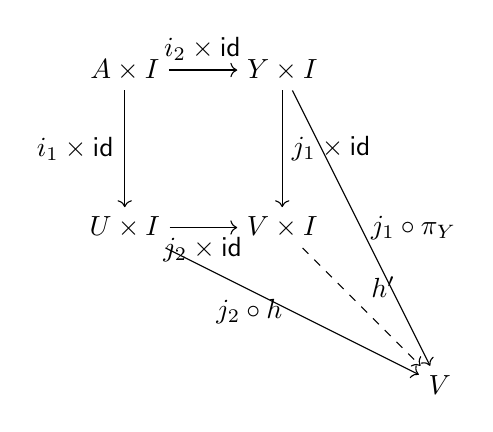
\begin{tikzpicture}
\node (D1) at (0,2) [] {$A\times I$};
\node (D3) at (2,2) [] {$Y\times I$};
\node (D5) at (2,0) [] {$V\times I$};
\node (D7) at (0,0) [] {$U\times I$};
\node (D9) at (4,-2) [] {$V$};

\draw [->] (D1) -> (D3) node[midway, above] {$i_2\times \id{}$};
\draw [->] (D3) -> (D5) node[midway, right] {$j_1\times \id{}$};
\draw [->] (D7) -> (D5) node[midway, below] {$j_2\times \id{}$};
\draw [->] (D1) -> (D7) node[midway, left] {$i_1\times \id{}$};

\draw [->] (D3) -> (D9) node[midway, right] {$j_1\circ \pi_Y$};
\draw [dashed, ->] (D5) -> (D9) node[midway, above right] {$h'$};
\draw [->] (D7) -> (D9) node[midway, left] {$j_2\circ h$};
\end{tikzpicture}
\end{center}
Definiere $r' : V \pfeil{}j_1(Y)$ durch $r' = h'(\_, 1)$\\
Dann ist $h' : \id{} \simeq j_1\circ r$ relativ zu $j_1(Y)$.
\end{Beweis}

\section{Noch mehr Anwendungen des Satzes von Seifert-van Kampen}

\Satz{}
Sei folgender Pushout gegeben, wobei $A, X, Y$ wegzusammenhängend sind:
\begin{center}
\begin{tikzpicture}
\node (D1) at (0,2) [] {$A$};
\node (D3) at (2,2) [] {$Y$};
\node (D5) at (2,0) [] {$Z$};
\node (D7) at (0,0) [] {$X$};

\draw [right hook->] (D1) -> (D3) node[midway, above] {$i_2$};
\draw [->] (D3) -> (D5) node[midway, right] {$j_1$};
\draw [->] (D7) -> (D5) node[midway, below] {$j_2$};
\draw [right hook->] (D1) -> (D7) node[midway, left] {$i_1$};
\end{tikzpicture}
\end{center}
wobei $i_1, i_2$ Einbettungen und $A \abg X, \abg Y$ ein Nachbarschaftsdeformationsretrakt sind.
Dann erhalten wir folgenden Pushout in $\Grp$ für alle $x \in A$:
\begin{center}
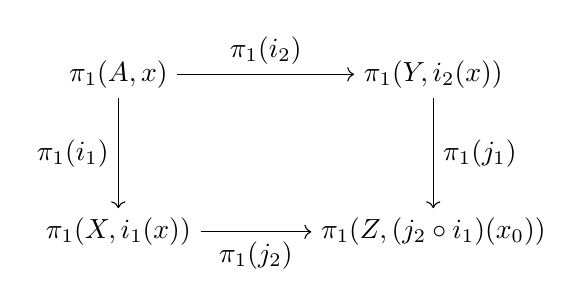
\begin{tikzpicture}
\node (D1) at (0,2) [] {$\pi_1(A,x)$};
\node (D3) at (4,2) [] {$\pi_1(Y,i_2(x))$};
\node (D5) at (4,0) [] {$\pi_1(Z,(j_2\circ i_1)(x_0))$};
\node (D7) at (0,0) [] {$\pi_1(X, i_1(x))$};

\draw [->] (D1) -> (D3) node[midway, above] {$\pi_1(i_2)$};
\draw [->] (D3) -> (D5) node[midway, right] {$\pi_1(j_1)$};
\draw [->] (D7) -> (D5) node[midway, below] {$\pi_1(j_2)$};
\draw [->] (D1) -> (D7) node[midway, left] {$\pi_1(i_1)$};
\end{tikzpicture}
\end{center}

\begin{Beweis}{}
Betrachte folgende Deformationsretrakte
\begin{align*}
X \overset{o}{\supset} U_x \Pfeil{r_x} A && h_x : \id{} \simeq i_1 \circ r_x \text{ relativ zu A}\\
Y \overset{o}{\supset} U_y \Pfeil{r_y} A && h_y : \id{} \simeq i_2 \circ r_y \text{ relativ zu A}\\
\end{align*}
Definiere folgende Verdickungen von $A,X,Y$ in $Z$:
\begin{align*}
V_A := U_X \cup U_Y && V_X := X \cup U_Y && V_Y := Y \cup U_X
\end{align*}
Dann sind $X \subset V_X, Y \subset V_Y, A \subset V_A$ Deformationsretrakte. Es ergibt sich folgende Situation
\begin{center}
\diag{V_A}{}{V_X}{}{Z}{}{V_Y}{}
\end{center}
woraus sich ein Pushout für die entsprechenden Fundamentalgruppen ergibt. Aufgrund der Deformationsretrakte gilt aber
\begin{align*}
\pi_1(V_A) = \pi_1(A) && \pi_1(V_X) = \pi_1(X) && \pi_1(V_Y) = \pi_1(y)
\end{align*}

\end{Beweis}

%	13.05.15, 10.VL
\Bsp{}
$X = S^1\times [0,1]/\sim$, $\sim$ generated by
\[(z,0) \sim (e^{2\pi /n}z,0) ; (z,1) \sim (e^{2\pi /m}z,1) \]
identifying points that are  an angle $2\pi /n$, $2\pi/m$ apart\\
It follows:
\[top \cong S^1; bottom \cong S^1 \]
Pushout: (1)\\

The inclusions
\[top \hookrightarrow X_{T}, bottom \hookrightarrow X_B \]
are deformation retracts, in particular homotopy equivalences.\\

In the first case,
\[r: X_T \longrightarrow Top, [(z,t)] \longmapsto [(z,1)]\]
\[h: X_T\times [0,1]\longrightarrow X_T, ([(z,s)],t) \longmapsto [(z,s\cdot t)] \]
provides the data of a deformation retract. Similiar for bottom.\\

van Kampen yields a pushout of groups, when applying $\pi_1$ to (1).
(2)\\

How do the induced morphisms look like?\\
In the case of top:
\[r_* : \pi_1(X_T) \longrightarrow \pi_1(Top), \gamma \longmapsto \gamma^n \]m
One gains
\[\pi_1(S^1\times \{\frac{1}{2}\}) \longrightarrow \pi_1(X_T) \overset{\sim}{\longrightarrow} \pi_1(Top) \overset{\sim}{\longrightarrow} \pi_1(S^1) \cong \Z  \]
Be $\gamma$ a generator of $\pi_1(Top)$, $r$ applied to the generator of $\pi_1(S^1\times \frac{1}{2})$ wraps around $m$ times the top circle.\\

Because of (2) we obtain a group presentation
\[\pi_1(X) \cong \left\langle a,b~|~a^m = b^n \right\rangle \]
We have an epimorphism
\[\pi_1(X) \longrightarrow > \Z/m \star \Z /n \]
\[a \longmapsto 1_{\Z/m}\]
\[b \longmapsto 1_{\Z/n}\]

\newpage

\chapter{Homology - the axiomatic approach 2}

\section{2.1 The Eilenberg-Steenrod axioms}
Let $R$ be a commutative Ring.\\

A sequence of moprhisms of $R$-modules
\[M_{i+1} \overset{f_{i+1}}{\longrightarrow} M_i \overset{f_{i}}{\longrightarrow} M_{i-1} \overset{f_{i-1}}{\longrightarrow}\]
is called \df{exact} if
\[Kern f_i = im f_{i+1} \forall i\]

\subsubsection{Definition}
A \df{homology theory} $(H_*, \partial_*)$ with values in $R$-modules consists of a family $(H_n)_{n\in\Z}$ of functors
\begin{align*}
H_n : \Top^2 & \longrightarrow R-\Mod
\end{align*}
from the category of pairs of spaces to the category of $R$-modules and a family of natural transformations $(\partial_n)_{n\in \Z}$
\[\partial_n : H_n \longrightarrow H_{n-1} \circ J \]
where $J$ is the functor 
\[J : \Top^2 \longrightarrow \Top^2\]
\[(X,A) \longmapsto (A,\emptyset)\]
such that the following axioms are true
\begin{itemize}
\item \df{Homotopy invariance}\\
If $f,g : (X,A) \rightarrow (Y,B)$ are maps of pairs of spaces and $h_t : f \backsimeq g$ is a homotopy with $h_t(A) \subset B \forall t \in [0,1]$ then
\[H_n(f) = H_n(g)\]
\item \df{Long exact sequence}\\
For every  pair $(X,A)$ the following sequence of $R$-modules is exact:
\[ \ldots\longrightarrow H_{n+1}(X,A)\overset{\partial_{n+1}(X,A)}{\longrightarrow }H_n(A,\emptyset)\overset{H_n(\iota)}{ \longrightarrow} H_n(X,\emptyset) \overset{H_n(j)}{ \longrightarrow}H_n(X,A) \longrightarrow H_{n-1}(A,\emptyset) \longrightarrow \ldots \]
is exact where
\[\iota : (A,\emptyset) \longrightarrow (X,\emptyset) \]
\[j : (X,\emptyset) \longrightarrow (X,A)\]
This maps $\partial_i(X,A)$ are called \df{boundary homomorphisms}.

\item \df{Excision axiom}\\
Let $X$ be a space and $A,B\subset X$ be a subspace such that $\overline{A} \subset B^o$. Then the $R$-homomorphisms
\[H_n(X\setminus A, B\setminus A) \longrightarrow H_n(X,B)\]
induced by
\[(X\setminus A, B\setminus A) \hookrightarrow (X,A)\]
is an isomorphism for all $n$.

\end{itemize}
If $(H_*, \partial_*)$ in addition satisfies the following, we say  $(H_*, \partial_*)$ satisfies the \df{dimension axiom}:
\[H_n(\{*\}, \emptyset) \cong R, if n = 0; 0 if n \neq 0\]

Notation: In the sequel we write $H_n(X)$ instead of $H_n(X,\emptyset)$.

\subsubsection{Remark}
In a nutshell, $(H_*, \partial_*)$ is the following:
\begin{itemize}
	\item $(X,A) \rightsquigarrow R-\text{Modules} H_n(X,A), n \in \Z$
	\item $(X,A) \overset{f}{\rightarrow} (Y,B) \rightsquigarrow H_n(X,A) \overset{H_n(f)}{\rightarrow} H_n(Y,B)$
	\item boundary homom. (3)
\end{itemize}

\subsubsection{Remark}
Long exact sequence for $(X,X)$
\[H_{n+1}(X,X) \overset{\partial_{n+1}}{\longrightarrow} H_n(X) \overset{\sim}{\longrightarrow} H_n(X) \overset{H_nj}{\longrightarrow} H_n(X,X)\overset{\partial_{n}}{\longrightarrow} H_{n-1}(X) \overset{\sim}{\longrightarrow} H_{n-1}(X)  \]

\[Kern id = im(\partial_n) = 0 \Longrightarrow \partial_n = 0 \]
\[im H_n(j) = Kern \partial_n = Hn(X,X)\]
\[Ker H_n(j) = im id = H_n(X) \]
Therefore $H_n(X,X) = 0$

\section{2.2 First conclusions from the axioms}
\Satz{Fünferlemma}
Consider the following commuting diagram of $R$-modules
(4)
such that both rows are exact and $f_1$ is surjective, $f_5$ is injective and $f_2$ and $f_4$ are isomorphisms. Then $f_3$ is an isomorphism.

\paragraph{Proof by Diagrammjagd}

% % 11.VL 18.5.15

Im folgenden ist $(H_n,\partial_n)$ eine Homologietheorie, die nicht zwangsläufig das Dimensionsaxiom erfüllt.

\Kor{}
Sei $(X,A) \pfeil{f} (Y,B)$ ein Pfeil. Sind $H_n(X) \pfeil{H_n(f)} H_n(Y)$ und $H_n(A) \pfeil{H_n(f)} H_n(B)$ isomorph für alle $n$, so ist es auch $H_n(X,A) \pfeil{H_n(f)} H_n(Y,B)$ für alle $n$.

\Lem{}
Seien $A \subset B \subset X$ topologische Räume; dann existiert eine natürliche lange Sequenz (die sogenannte \df{Dreier-Sequenz})
\[\Pfeil{} H_{n+1}(X,A) \Pfeil{} H_{n+1}(X,B) \Pfeil{\d_{n+1}(X;B,A)} H_n(B, A) \Pfeil{} H_n(X,A) \Pfeil{} \]
induziert durch die Inklusionen
\[ (B, A) \Inj{i} (X,A) \Inj{j} (X,B) \]
\begin{Beweis}{}
Definiere
\[\d_n(X;B,A) = H_{n-1}(l) \circ \d_n(X, B) \]
wobei $(B,\emptyset) \Inj{l} (B,A) $
\end{Beweis}

\Def{Excisive Triad}
Seien $X_1,X_2 \subset X$ Räume. $(X, X_1, X_2)$ heißt ein \df{Schneidungs-Trias}, falls die Inklusion
\[(X_1, X_1\cap X_2) \Inj{} (X, X_2)\]
einen Isomorphismus
\[H_n(X_1, X_1\cap X_2) \Pfeil{} H_n(X, X_2)\]
für alle $n$ induziert.

\Bem{}
Sind $X_1,X_2 \off X$ und $X = X_1\cup X_2$, dann ist $(X, X_1, X_2)$ aufgrund des Excision-Axioms excisiv.

\Satz{Mayer-Vietoris}
Sei $(X,X_1,X_2)$ ein excisives Trias. Sei $A \subset X_0 = X_1\cap X_2$. Dann existiert eine natürliche exakte Sequenz (sogenannte \df{Mayer-Vietoris Sequenz})
\[ \pfeil{} H_{n+1}(X_1,A) \oplus H_{n+1}(X_2,A) \pfeil{H_{n+1}(j_1) - H_{n+1}(j_2)} H_{n+1}(X,A) \pfeil{\d_{n+1}} H_{n}(X_0,A) \pfeil{H_n(i_1) + H_n(i_2)} H_{n}(X_1,A) \oplus H_{n}(X_2,A) \pfeil{} \]
induziert durch die Inklusionen
\begin{align*}
(X_0,A) \inj{i_1} (X_1,A) \inj{j_1} (X,A) && (X_0,A) \inj{i_2} (X_2,A) \inj{j_2} (X,A)
\end{align*}

% % % 12.VL, 22.5

\Satz{Mayer-Vietoris für Pushouts}
Sei
\begin{center}
\diag{A}{f}{Y}{j}{Z}{g}{X}{i}
\end{center}
ein Pushout, wobei $A \inj{i} X$ die Einbettung eines abgeschlossenen Teilraumes und $A \subset X$ ein NDR ist.\\
Dann induziert $(f,g) : (X,A) \pfeil{} (Z,Y)$ Isomorphien
\[H_n(X,A) \pfeil{\cong} H_n(Z,Y) \]
Ferner existiert folgende natürliche exakte Sequenz (\df{Mayer-Vietoris Sequenz})
\[ \pfeil{} H_{n+1}(Z) \pfeil{\d_{n+1}} H_n(A) \pfeil{H_n(i) + H_n(f)} H_n(X) \oplus H_n(Y) \pfeil{H_n(g) - H_n(j)} H_n(Z) \]



Ab sofort fordern wir, dass unsere Homologietheorie das Dimensionsaxiom erfüllt.

\Bem{}
Für alle $n \geq 1$
\begin{align*}
H_i(S^n) =\left\lbrace \begin{aligned}
R && i = n \text{ oder } i = 0\\
0 && \text{ sonst}
\end{aligned}
\right.
\end{align*}
und
\begin{align*}
H_i(S^0) =\left\lbrace \begin{aligned}
R\oplus R && i = 0\\
0 && \text{ sonst}
\end{aligned}
\right.
\end{align*}

\section{Grade der Selbstabbildungen der Sphäre}
In diesem Kapitel erfüllt unsere Theorie das Dimensionsaxiom.

\Def{Reduzierte Homologie}
Definiere die \df{reduzierte Homologie} durch
\[\H_n(X) := \Ker(H_n(X) \pfeil{} H_n(\bullet)) \]
Dann gelten
\begin{itemize}
\item $\H$ ist funktoriell.
\item $\H_n(X) = H_n(X) \Longleftrightarrow  n \neq 0$ 
\item $H_n(X) = R\oplus \H_n(X) \Longleftrightarrow  n = 0$ 
\end{itemize}

\Def{Grad}
Sei $R = \Z$, $n \geq 0$. Dann ist der \df{Grad} einer Abbildung $S^n\pfeil{f}S^n$ definiert als die eindeutig bestimmte Zahl $\deg f \in \Z$, die folgendes Diagramm zum kommutieren bringt:
\begin{center}
\diag{\H_n(S_n)}{\H_n(f)}{\H_n(S_n)}{\cong}{\Z}{\cdot \deg f}{\Z}{\cong}
\end{center}

\Bem{}
\begin{itemize}
\item Ist das Bild von $f$ null-homotop, so ist $\deg f = 0$.
\item $\deg(f\circ g) = \deg f \cdot \deg g$
\item $\deg \id{S^n} = 1$
\item Der Grad ist unabhängig von der Wahl der Homologietheorie.
\end{itemize}

\Lem{}
Sei
\begin{align*}
f : S^n & \longrightarrow S^n\\
(x_0, \ldots, x_i, \ldots, x_n) & \longmapsto (x_0, \ldots, -x_i, \ldots, x_n)
\end{align*}
Dann ist
\[ \deg f = -1 \]

\Satz{}
Sei $n\geq 2$ gerade, $S^n \pfeil{f} S^n$. Dann existiert ein $x$ mit
\[f(x) \in \set{x, - x}{} \]

\Satz{}
Sei $n\geq 2$ gerade. Dann existiert für jedes stetige Vektorfeld auf $S^n$ mindestens ein Verschwindungspunkt.

\Satz{}
Sei $A \in \R^{n+1 \times n+1}$ regulär.
\[\deg (x\mapsto \frac{Ax}{||Ax||}) = sign(\det A) \]

\Satz{}
Die Abbildung $S^1\pfeil{z \mapsto z^k} S^1$ hat Grad $k$

\Satz{}
Sei $f : S^n \pfeil{} S^n$ differenzierbar. $q \in S^n$ regulärer Punkt, $f\i(q) = \set{p_1,\ldots, p_k}{}$. $d_i = sign(\det f'(p_i))$, wobei die Jacobimatrix durch Karten von $p_i$ und $q$ berechnet wird, die sich um ein Element aus $SO(n+1)$ unterscheiden.
\[\deg f = \sum_i d_i \]

\Kor{}
Der Grad ist unabhängig von der Wahl der Homologietheorie.

\Lem{}
Sei $g : S^n \pfeil{} S^n$ glatt, $q$ ein regulärer Punkt, sodass $g\i = p$.\\
Dann ist der Grad von $g$ das Vorzeichen der Determinante der Jacobimatrix von $g$ bei $p$, berechnet durch Karten, die sich ausschließlich um eine Rotation unterscheiden.

\chapter{The construction of singular homology}

\section{Algebraische Vorbereitungen}
Sei $R$ ein kommutativer Ring mit 1.

\Def{Kettenkomplex}
Ein $R$-\df{Kettenkomplex} ist eine Familie von $R$-Moduln $(C_n)_{n\in \Z}$ mit Pfeilen $c_n : C_n \pfeil{} C_{n-1}$, sodass $c_{n-1}\circ c_n = 0$.\\
Ein Pfeil $f : C_n \rightarrow D_n$ von $R$-{Kettenkomplexen} ist eine Familie von Modulmorphismen $f_n : C_n \pfeil{} D_n$, sodass die sich ergebenden Diagramme kommutierten.

\Def{Homologie}
Die $n$-te Homologie eines Kettenkomplexes ist definiert durch
\[ H_n(C_*,c_*) := \Ker(c_n)/ \Img c_{n+1} \]
Elemente $c \in \Ker c_n$ heißen \df{Zykel}, $b \in \Img c_{n+1}$ heißen \df{Ränder}. Zwei Zykel, die sich nur um einen Rand unterscheiden, heißen \df{homolog}.

\Bem{}
Eine Kettenabbildung $f : C_n \rightarrow D_n$ induziert einen wohldefinierten Pfeil von $R$-Moduln $H_n(f) : H_n(C_n) \pfeil{} H_n(D_n) $ durch $H_n(f)([c]) = [f(c)]$. Insofern ist $H_n$ ein Funktor $R-\textbf{Chain} \pfeil{} R-\Mod$.

\Def{Homotopie}
Eine \df{Kettenhomotopie} zwischen Kettenpfeilen $f_n, g_n : C_n \pfeil{} D_n$ ist eine Familie von Modulmorphismen $h_n : C_n \pfeil{} D_{n+1}$, sodass
\[ f_n - g_n = d_{n+1}h_n + h_{n+1}c_n \]
Man schreibt in diesem Fall $f\simeq g$

\Lem{}
Zwei homotope Pfeile von Kettenkomplexen induzieren in der Homologie dieselbe Abbildung.

\Bem{}
\begin{itemize}
\item Ketten-Homotopie ist eine Äquivalenzrelation
\item Ketten-Homotopie ist verträglich mit der Verkettung von Pfeilen.
\end{itemize}

\Def{}
Eine Sequenz von Kettenkomplexen
\[A \pfeil{} B \pfeil{} C \]
heißt \df{exakt}, falls sie gradweise \df{exakt} ist
\[ A_n \pfeil{} B_n \pfeil{} C_n \]

\Satz{}
Sei folgende kurze exakte Sequenz von Kettenkomplexen gegeben
\[0 \Pfeil{} C_* \Pfeil{i_*} D_* \Pfeil{p_*} E_* \Pfeil{} 0 \]
Dann existiert folgende natürliche lange exakte Sequenz in der Homologie
\[ \Pfeil{} H_{n+1}(E_*) \Pfeil{\d_{n+1}} H_n(C_*) \Pfeil{H_n(i_*)} H_n(D*) \Pfeil{H_n(p_*)} H_n(E*) \Pfeil{\d_n} H_{n-1}(C_*) \Pfeil{}  \]

\section{Definition der singulären Homologie}

\Def{}
Der \df{Standard $n$-Simplex} ist definiert als
\[\Delta_n := \set{x \in \R^{n+1}}{||x||_1 = 1, x_i \geq 0} \]

\Def{}
Sei $X$ ein top. Raum. Ein \df{singulärer $n$-Simplex} ist ein Abbildung
\[ \delta : \Delta_n \Pfeil{} X \]
Die Menge aller singulärer $n$-Simplizes wird durch $s_n(X)$ bezeichnet.

\Def{}
Sei $X$ ein Raum, definiere die \df{$n$-te singuläre Kettengruppe} als den freien $R$-Modul mit Basis $s_n(X)$:
\begin{align*}
\Cs{n}(X;R) := \left\lbrace
\begin{aligned}
R[s_n(X)] && n \geq 0\\
0 && n < 0
\end{aligned}
\right.
\end{align*}

\Def{}
Definiere die \df{$k$-te Facette} eines Simplex durch
\func{i^n_k}{\Delta_{n-1}}{\Delta_n}{(x_1,\ldots, x_n)}{(x_1, \ldots, x_{k-1}, 0, x_k,\ldots, x_{n})}

\Def{}
Wir machen aus $\Cs{*}(X;R)$ einen Kettenkomplex, indem wir folgende Differentiale einführen
\func{\cs{n}(X;R)}{\Cs{n}(X;R)}{\Cs{n-1}(X;R)}{\delta}{\sum_{k = 1}^{n+1}(-1)^k\delta \circ i^n_k(\delta) }

\Lem{}
$\cs{n} \circ \cs{n+1} = 0$, d.h. $(\Cs{n}, \cs{n})$ ist ein Kettenkomplex.

\Bem{}
$\Cs{*}$ ist ein Funktor von \Top zu $R$-\textbf{Ketten}, wobei für $f : X\pfeil{} Y$
\[ \Cs{n}(f)(\delta) = f \circ \delta \]
Sei $A \inj{i} X$ die Inklusion eines Teilraumes, definiere
\[ \Cs{n}(X, A; R) := \Coker (\Cs{n}(i))  = \Cs{n}(X;R) /\Img \Cs{n}(i) \]
Die Differentiale $\cs{*}(X;R)$ machen aus $\Cs{*}(X,A;R)$ einen Kettenkomplex.

\Def{}
Für ein Paar $(X,A)$ definieren wir die \df{$n$-te singuläre Homologie} durch
\[\Hs{n}(X,A;R) := H_n(\Cs{*}(X,A;R)) \]

\Satz{}
$(\Hs{*}(\_,R), \d_*)$ ist eine Homologietheorie mit Koeffizienten in $R$, die das Dimensionsaxiom erfüllt.

\section{Verifikation der Eilenberg-Steenrod Axiome}

\subsection{Homotopie Invarianz}
Sei $i_t : x \mapsto (x,t)$. Wir konstruieren eine natürliche Homotopie
\[ h_*(X) : \Cs{*}(i_0) \simeq \Cs{*}(i_1) \]
sodass
\begin{enumerate}
\item $h_n(X) : \Cs{n}(X; R) \longrightarrow \Cs{n+1}(X\times I; R) $
\item $\cs{n+1}(X\times I) \circ h_n(X) + h_{n-1}(X) \circ \cs{n}(X) = \Cs{n}(i_0) - \Cs{n}(i_1) $
\item Für alle $g : X \pfeil{} Y$ kommutiert
\begin{center}
\Diag{\Cs{n}(X;R)}{h_n(X)}{\Cs{n+1}(X\times I;R)}{\Cs{n+1}(g\times \id{I})}{\Cs{n+1}(Y \times I;R)}{h_n(Y)}{\Cs{n}(Y;R)}{\Cs{n}(g)}
\end{center}
\end{enumerate}

$h_*(X)$ ist eindeutig bestimmt durch
\begin{center}
\Diag{\Cs{n}(\Delta_n;R)}{h_n(\Delta_n)}{\Cs{n+1}(\Delta_n\times I;R)}{\Cs{n+1}(\delta\times \id{I})}{\Cs{n+1}(X \times I;R)}{h_n(X)}{\Cs{n}(X;R)}{\Cs{n}(\delta)}
\end{center}

\subsection{Ausschneidung}
\Def{}
Sei $(U_i)_{i\in I}$ eine Überdeckung von $X$. $\delta \in s_n(X)$ heißt \df{$U$-klein}, falls $\Img \delta \subset U_i$.
Sei $C^U_*(X; R) \subset \Cs{*}(X;R)$ der Unterkettenkomplex, der durch die $U$-kleinen Simplizes generiert wird.

\Lem{Kleine Simplizes Lemma}
$C^U_*(X;R) \inj{} \Cs{*}(X;R)$ induziert Isomorphien auf allen Homologiemoduln.

Zeige durch die Überdeckung $U = \set{B, X - A}{}$, dass $\Hs{*}(X, B; R) \cong \Hs{*}(X - A, B - A; R)$

\subsection{Additivität}
Für jede Homologie gilt
\[H_*(\bigsqcup^n_{i= 1} X_i ) = \bigoplus_{i=1}^nH_*(X_i) \]
\Def{}
Eine Homologie erfüllt das \df{Additivitätsaxiom}, falls für jede Menge $I$ gilt
\[H_*(\bigsqcup_{i\in I} X_i ) = \bigoplus_{i\in I}H_*(X_i) \]
Die singuläre Homologie erfüllt das Additivitätsaxiom.

\section{Singuläre Homologie in den Graden 0 und 1}
\Def{}
Definiere die \df{Vergrößerungsabbildung}
\func{\e}{\Cs{0}(X;R)}{R}{\sum n_xx}{\sum n_x}
Dann ist $\e = 0$ auf $\Img \cs{1}$ und induziert einen Homomorphimus
\[ \e : \Cs{0}(X;R)/\Img \cs{1} = \Hs{0}(X;R) \Pfeil{} R  \]

\Satz{}
Ist $X \neq \emptyset$ wegzusammenhängend, so ist 
\[ \e :  \Hs{0}(X;R) \Pfeil{} R  \]
ein Isomorphismus.

\Kor{}
$\Hs{0}(X;R)$ ist ein freier $R$-Modul mit $\pi_0(X)$ als Basis.

\Satz{Hurewicz' Satz in Grad 1}
Die Abbildung
\func{h}{\pi_1(X,x_0)}{\Hs{1}(X;\Z)}{[f]_\sim}{[f]}
ist ein wohldefinierter Gruppenhomomorphismus.\\
Ist $X$ wegzusammenhängend, so ist $h$ surjektiv und $\Ker h = [\pi_1(X,x_0),\pi_1(X,x_0)]$

\chapter{Applications of singular homology}
Im folgenden betrachten wir ausschließlich die singuläre Homologie.

\section{Fundamentalsatz der Algebra}

\Satz{Fundamentalsatz der Algebra}
Jedes nichtkonstante Polynom über $\mathbb{C}$ hat eine Nullstelle in $\mathbb{C}$.

\section{Das Theorem von Borsuk-Ulam}

\Satz{Borsuk-Ulam}
Für jede stetige Abbildung $f : S^n \pfeil{} \R^n$ existiert ein $x \in S^n$, sodass
\[f(x) = f(-x) \]

\Satz{Ham Sandwich theorem}
Seien $A_1, \ldots, A_n \subset \R^n$ Borelmengen mit endlichem Lebesguemaß $\lambda(A_i) < \infty$. Dann existiert eine Hyperebene, die jedes $A_i$ maßtechnisch halbiert.

\Satz{Äquivarianz Theorem}
Sei $g : S^n \rightarrow S^m$ dergestalt, dass
\[g(-x) = -g(x) \forall x \in S^n\]
Dann ist $n \leq m$

\section{Invarianz der Dimension}
\Satz{}
\[\R^n \cong \R^m \Longleftrightarrow n = m \]

\section{Browers Fixpunktsatz}
\Satz{}
Sei $n\geq0$. Jede stetige Abbildung $f : D^n \rightarrow D^n$ hat einen Fixpunkt.


\chapter{CW-complexes and cellular homology}

\section{CW-Komplexe}
\Def{}
Eine \df{$k$-dimensionale Zelle} $e \subset X$, die bzgl. ihrer Spurtopologie homöomorph zu $E^k= \overset{o}{D^k}$ ist. Jeder Punkt in $X$ ist eine 0-Zelle.

\Def{}
Ein \df{Whitehead Komplex} ist ein Raum $X$ zusammen mit einer Zellzerlegung $(e_i)_{i\in I}$, sodass
\begin{itemize}
\item $\overset{.}{\bigcup}_{i\in I}e_i = X$
\item $X$ ist Hausdorff
\item Für jede $n$-Zelle $e_i$ existiert eine Abbildung $\Phi : D^n \pfeil{} X$, sodass $\Phi_{|E^n} : E^n \pfeil{\cong} e_i$ ist und  $\Phi(S^n)$ in der Vereinigung der $\leq n -1$-Zellen liegt.
\item \paragraph{Closure finiteness} Der Abschluss einer Zelle schneidet sich nur mit endlichen vielen Zellen.
\item \paragraph{Weak topology} 
\[A \abg X \Longleftrightarrow A\cap \overline{e_i} \abg \overline{e_i} ~~\forall i \in I  \]
\end{itemize}

\Def{}
Eine Teilmenge $A \subset X$ eines Whitehead Komplexes heißt ein \df{Subkomplex}, falls es eine Vereinigung von Zellen ist und der Abschluss jeder Zelle von ihr in $A$ liegt.

\Bem{}
$\Phi(D^n) = \overline{e_i}$

\Satz{}
Sei $X$ ein Whitehead Komplex.
\begin{itemize}
\item Eine kompakte Teilmenge $K \subset X$ schneidet nur endlich viele Zellen.
\item Ein endlicher Subkomplex (besteht nur aus endlich vielen Zellen) ist kompakt in $X$.
\item Ist $L\subset X$, so bezeichnet $X(L)$ den kleinsten Subkomplexen, der $L$ enthält. Dann ist $X(e) = X(\overline{e})$ ein endlicher Subkomplex für jede Zelle $e$.
\item Jede kompakte Teilmenge von $X$ ist in einem endlichen Subkomplexen enthalten.
\item
\[A \abg X \Longleftrightarrow A\cap L \abg L ~~\forall L : \text{ endlicher Subkomplex}  \]
\item Jeder Subkomplex ist abgeschlossen.
\end{itemize}

\Satz{}
Ein Subkomplex eines Whitehead-Komplexes ist ein Whitehead-Komplex.

\Lem{Hilfslemma}
Sei folgendes Diagramm mit abgeschlossenen Einbettungen $j,J$ gegeben.
\begin{center}
\diag{A}{f}{Y}{J}{Z}{F}{X}{j}
\end{center}
$F$ soll eine Bijektion $X -A \Pfeil{} Z -Y$ induzieren. Ferner soll $F(X) \abg Z$ und $F : X \pfeil{} F(X)$ eine Identifikation sein.\\
Dann ist das obige Diagramm ein Pushout.

\Def{}
Definiere das $n$-Skelett eines Whitehead-Komplexes
\[X^n = \bigcup_{i=0}^n \bigcup_{e : \text{ i-Zelle}}e \]

\Satz{}
Sei $X$ ein Whitehead-Komplex
\begin{itemize}
\item $X$ trägt die \df{Kolimes-Topologie}, d.h.
\[ A \abg X \Longleftrightarrow A\cap X^i \abg X^i ~~\forall i  \]
\item Sei $(e_i)_{i\in I(n)}$ eine Familie von $n$-Zellen in $X$ mit charakteristischen Abbildungen $\Phi_i : D_i^n \rightarrow e_i$ und Einschränkungen $\varphi_i = \Phi_{i|S^{n-1}_i}$. Dann ist folgendes Diagramm ein Pushout
\begin{center}
\Diag{\Coprod{i\in I(n)}S^{n-1}_i }{\Coprod{i\in I(n)}\varphi_i}{X^{n-1}}{}{X^n}{\Coprod{i\in I(n)}\Phi_i}{\Coprod{i\in I(n)}D^{n-1}_i }{}
\end{center}
\end{itemize}

\Def{}
Sei $A \subset X$, eine \df{CW-Zerlegung} von $(X,A)$ besteht aus einer Filtration von Teilräumen
\[ A \subset X^{-1} \subset X^0 \subset X^1 \subset \ldots \subset X = \bigcup_i X_i \]
sodass
\begin{itemize}
\item $X$ trägt die {Kolimes-Topologie}
\item Für jedes $n \geq 0$ existiert folgender Pushout
\begin{center}
\Diag{\Coprod{i\in I(n)}S^{n-1} }{}{X^{n-1}}{}{X^n}{}{\Coprod{i\in I(n)}D^{n-1}}{}
\end{center}
\end{itemize}
Ein Paar $(X,A)$ zusammen mit einer CW-Zerlegung heißt ein \df{relativer CW-Komplex}. Ist $A = \emptyset$, so nennt man $X$ einfach \df{CW-Komplex}. Ein Raum mit einer CW-Zerlegung heißt auch \df{CW-Raum}. Die \df{zelluläre Dimension} von $(X,A)$ ist definiert als das kleinste $n \in \N\cup\{0,\infty\}$, sodass $X^{n} = X^{n+1}$.

\Satz{}
Jeder Whitehead Komplex ist ein CW-Komplex und umgekehrt.

\Satz{}
Sind $X$ und $Y$ CW-Komplexe, von denen mindestens einer lokal kompakt ist, so ist $X \times Y$ ebenfalls ein CW-Komplex, wobei
\[ (X \times Y)^n = \bigcup X^i \times Y^{n-i}  \]

\Def{}
Eine \df{zelluläre Abbildung} $f : (X,A) \pfeil{} (Y,B)$ ist eine stetige Abbildung, sodass
\[ f(X^n) \subset Y^n \]

\section{Zelluläre Homologie}
\Def{}
Sei $(X,A)$ ein relativer CW-Komplex. Definiere den \df{zellulären Kettenkomplex} $\Cw{*}(X,A;R)$ durch
\[ \Cw{n}(X,A;R) := H^n(X^n, X^{n-1}; R)  \]
\[{\cw{n}}: {\Cw{n}(X,A;R)}\Pfeil{}{\Cw{n - 1}(X,A;R)}\]
wobei die Randmorphismen durch die Dreiersequenz des Tripels $X^{n-2} \subset X^{n-1} \subset X^n $ bestimmt werden.\\
Die Homologie
\[\Hw{n}(X,A; R) := H_n(\Cw{*}(X, A; R)) \]
wird \df{zelluläre Homologie} genannt.

\Satz{}
Es gibt Isomorhien (natürlich, unter Berücksichtigung der zellulären Struktur)
\[ \Hw{n}(X, A;R) \Pfeil{\cong} H_n(X,A;R) ~~~~ \forall n \geq 0 \]

\Def{}
Sei $(X,A)$ ein relativer CW-Komplex mit Pushouts
\begin{center}
\Diag{\Coprod{i\in I(n)}S^{n-1}_i }{\varphi^n = \Coprod{i\in I(n)}\varphi_i}{X^{n-1}}{}{X^n}{\Phi^n = \Coprod{i\in I(n)}\Phi_i}{\Coprod{i\in I(n)}D^{n-1}_i }{}
\end{center}
betrachte außerdem den Pushout
\begin{center}
\diag{S^{n-1}}{}{*}{}{S^n}{u_n}{D^{n}}{}
\end{center}
Definiere für $n \geq 2, i \in I(n), j\in I(n-1)$ die \df{Inzidenznummer} $\inc{n}{i,j} \in \Z$ als den Grad der Komposition
\begin{align*}
S^{n-1} \Pfeil{\varphi_i} X^{n-1} \Pfeil{} X^{n-1}/(X^{n-1} - e_j) \Pfeil{\Phi_j\i} D^{n-1}/S^{n-2} \Pfeil{u_{n-1}} S^{n-1}
\end{align*}
Für $n = 1$ definiere
\begin{align*}
\inc{1}{i,j} = \left\lbrace
\begin{aligned}
1 && \varphi_i(1) = e_j \text{ und } \varphi_i(-1) \neq e_j\\
-1 && \varphi_i(-1) = e_j \text{ und } \varphi_i(1) \neq e_j\\
0 && \text{ sonst}
\end{aligned}
\right.
\end{align*}
Definiere induktiv Erzeuger
\begin{align*}
s^n \in \H_n(S^n;R) && b^n \in H_n(D^n, S^{n-1}; R) 
\end{align*}
sodass
\begin{align*}
	[\delta^+] - [\delta^-] = s^0 & \in \H_0(S^0;R)                                                                 \\
	\d b^n = s^{n-1}              & \text{ wobei } \d : H_n(D^n, S^{n-1};R)\Pfeil{\cong} \H_{n-1}(S^{n-1};R)        \\
	s^n = H_n(u_n)(b^n)           & \text{ wobei } H_n(u_n)(b^n) : H_n(D^n, S^{n-1};R)\Pfeil{\cong} \H_{n}(S^{n};R)
\end{align*}

\Satz{}
Folgendes Diagramm kommutiert

\begin{center}
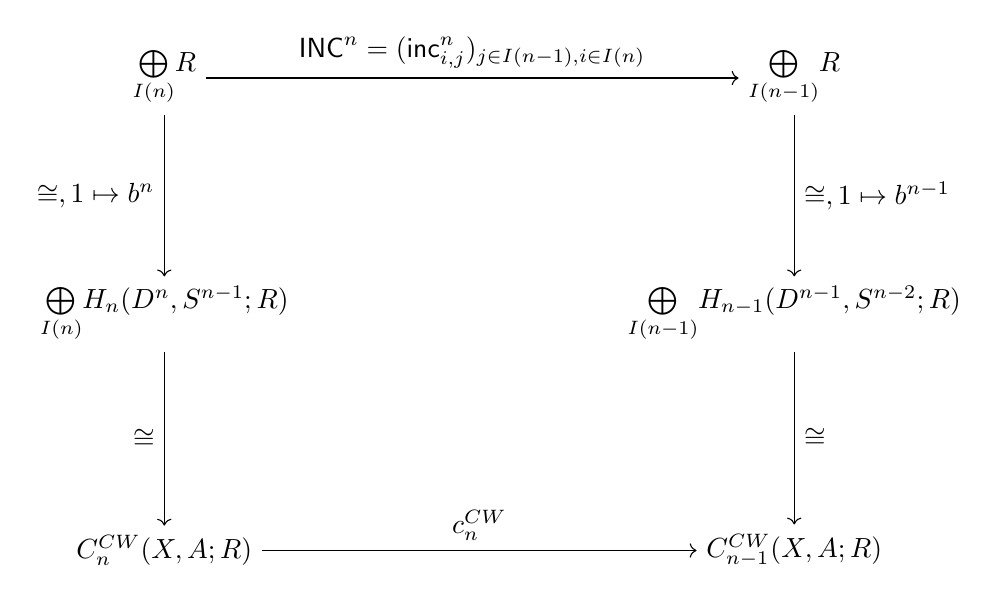
\begin{tikzpicture}
\node (D1) at (0,3) [] {$\Oplus{I(n)}R$};
\node (D3) at (8,3) [] {$\Oplus{I(n-1)}R$};
\node (D5) at (8,0) [] {$\Oplus{I(n-1)}H_{n-1}(D^{n-1}, S^{n-2}; R)$};
\node (D7) at (8,-3) [] {$\Cw{n-1}(X,A;R)$};
\node (D9) at (0,-3) [] {$\Cw{n}(X,A;R)$};
\node (D11) at (0,0) [] {$\Oplus{I(n)}H_{n}(D^{n}, S^{n-1}; R)$};

\draw [->] (D1) -> (D3) node[midway, above] {$\textsf{INC}^n = (\inc{n}{i,j})_{j\in I(n-1), i \in I(n)}$};
\draw [->] (D3) -> (D5) node[midway, right] {$\cong, 1 \mapsto b^{n-1}$};
\draw [->] (D5) -> (D7) node[midway, right] {$\cong$};
\draw [->] (D9) -> (D7) node[midway, above] {$\cw{n}$};
\draw [->] (D11) -> (D9) node[midway, left] {$\cong$};
\draw [->] (D1) -> (D11) node[midway, left] {$\cong, 1 \mapsto b^n$};
\end{tikzpicture}
\end{center}

\end{document}